\section{Cài đặt hệ thống}
\label{sec:impl}

\subsection{Tổ chức mã nguồn}

Toàn bộ mã nguồn được công khai tại \url{https://github.com/hotamago/nlp-efficient-rag}, viết bằng
Python 3.11 và quản lý môi trường bằng \texttt{uv} (khoá phiên bản trong \texttt{uv.lock}). Gói
\texttt{effrag} gồm các mô-đun:

\begin{itemize}
  \item \texttt{data.py}: đọc bộ NQ-Open 20 tài liệu, lấy mẫu cố định theo seed, gộp kho truy hồi.
  \item \nolinkurl{compression/}: lớp trừu tượng \texttt{Compressor} và \texttt{DocwiseCompressor}
  (ghi nhớ kết quả theo tập tài liệu), các bộ nén ở Bảng~\ref{tab:compressors} và bộ ghép
  \texttt{Chain} (nén nhiều tầng).
  \item \texttt{retrieval.py}: \texttt{BM25Retriever} và \texttt{DenseRetriever} (cắt Matryoshka,
  lượng tử int8/nhị phân, chỉ mục flat/HNSW).
  \item \texttt{generation.py}: client tương thích OpenAI, có cache theo hash của prompt và thử lại
  khi lỗi; cùng một mã chạy được với API thương mại, vLLM hoặc Ollama.
  \item \texttt{metrics.py}, \texttt{tokens.py}, \texttt{results.py}: chỉ số, bộ đếm token chung và
  lược đồ kết quả (CSV/JSONL) dùng chung cho cả nhóm.
  \item \nolinkurl{scripts/}: chạy thí nghiệm (\texttt{run\_compression.py}, \texttt{run\_retrieval.py},
  \nolinkurl{run_all_compression.sh}), vẽ hình (\texttt{make\_figures.py}); \nolinkurl{app/demo.py}: demo Gradio.
\end{itemize}

Thêm một bộ nén mới chỉ cần kế thừa \texttt{Compressor} và cài đặt một hàm:
\begin{lstlisting}[language=Python]
class MyPruner(DocwiseCompressor):
    name = "my_pruner"
    def _compress_docs(self, question, docs):   # -> one string per document ("" = drop)
        return [prune(question, d) for d in docs]
\end{lstlisting}

\subsection{Thư viện, mô hình và dữ liệu sử dụng}

\begin{table}[h]
\centering
\caption{Thành phần có sẵn được sử dụng.}
\label{tab:libs}
\small
\begin{tabularx}{\linewidth}{l X}
\toprule
Thành phần & Phiên bản / nguồn \\
\midrule
Dữ liệu & NQ-Open multi-document QA, 20 tài liệu~\cite{liu2024lost} (\nolinkurl{nelson-liu/lost-in-the-middle}) \\
LLM sinh câu trả lời & \nolinkurl{Qwen/Qwen2.5-7B-Instruct-AWQ}~\cite{qwen2025qwen25,lin2024awq}, phục vụ bằng vLLM 0.31~\cite{kwon2023vllm} \\
Nén token & \texttt{llmlingua} 0.2.2; \nolinkurl{microsoft/llmlingua-2-xlm-roberta-large-meetingbank}; \nolinkurl{Qwen/Qwen2.5-0.5B-Instruct} \\
Nén câu & \nolinkurl{naver/provence-reranker-debertav3-v1}; \nolinkurl{hotchpotch/open-provence-reranker-v1-gte-modernbert-base} \\
Truy hồi & \texttt{bm25s} 0.3, \texttt{faiss-cpu} 1.15, \texttt{sentence-transformers} 5.7; \nolinkurl{BAAI/bge-small-en-v1.5}, \nolinkurl{static-retrieval-mrl-en-v1}, \nolinkurl{cross-encoder/ms-marco-MiniLM-L6-v2} \\
Nền tảng & PyTorch 2.14, Transformers 4.57, tiktoken 0.14, Gradio 6 \\
\bottomrule
\end{tabularx}
\end{table}

\subsection{Thông số thực nghiệm}

\begin{itemize}
  \item \textbf{Phần cứng}: 1 GPU NVIDIA RTX 4070 SUPER 12GB, CPU 20 luồng (mặc định 4 luồng cho mỗi
  tiến trình, 8 luồng khi đo độ trễ CPU), 24GB RAM, WSL2.
  \item \textbf{Sinh câu trả lời}: Qwen2.5-7B-Instruct (lượng tử AWQ 4-bit), \texttt{temperature}=0,
  tối đa 100 token sinh (như \citet{liu2024lost}), độ dài ngữ cảnh tối đa 4.096 token.
  \item \textbf{Lấy mẫu}: 500 câu hỏi, seed 42, 3 vị trí đoạn vàng $\{1,10,20\}$.
  \item \textbf{Ngân sách nén}: tương ứng 2$\times$ ($\approx$1.450 token) và 4$\times$ ($\approx$730 token)
  so với $\approx$2.900 token của ngữ cảnh đầy đủ -- cùng hai mức của bảng kết quả LongLLMLingua.
  \item \textbf{LongLLMLingua}: \nolinkurl{condition_compare=True}, \nolinkurl{condition_in_question="after"},
  \nolinkurl{rank_method="longllmlingua"}, \nolinkurl{dynamic_context_compression_ratio=0.4},
  \nolinkurl{context_budget="+100"}, \nolinkurl{reorder_context="original"}.
  \item \textbf{LLMLingua-2}: \texttt{rate}$\in\{0{,}5; 0{,}25\}$, giữ bắt buộc ký tự xuống dòng, ``?'' và ``.''.
\end{itemize}

\paragraph{Điều chỉnh tương thích.} \texttt{llmlingua} 0.2.2 thao tác KV-cache dạng tuple cũ; chúng
tôi bọc hàm \texttt{forward} của LM để chuyển đổi qua lại với \texttt{DynamicCache} của Transformers
mới. Các mô hình Provence dùng mã tuỳ biến (\texttt{trust\_remote\_code}); với OpenProvence, mỗi cặp
(câu hỏi, đoạn) được đưa vào như một phần tử độc lập của batch.

\subsection{Demo}
\label{sec:demo}

\nolinkurl{app/demo.py} là ứng dụng Gradio chỉ gọi API của gói \texttt{effrag} (không sao chép logic),
gồm hai tab:
\begin{itemize}
  \item \textbf{So sánh bộ nén}: chọn một câu hỏi trong 200 câu đầu, vị trí đoạn vàng và các bộ nén;
  ứng dụng hiển thị số token trước/sau nén, thời gian nén, đáp án còn trong ngữ cảnh hay không và
  câu trả lời của LLM (Hình~\ref{fig:demo}). Với bộ nén theo đoạn, từng câu được giữ được tô xanh,
  câu bị loại bị gạch, đoạn vàng được đánh dấu (Hình~\ref{fig:demo-context}).
  \item \textbf{RAG end-to-end}: câu hỏi tự do $\to$ BM25S hoặc bge-small trên kho 50,7k đoạn
  $\to$ bộ nén $\to$ LLM.
\end{itemize}
Khi không có máy chủ LLM, demo vẫn chạy phần truy hồi và nén; mọi mô hình nén chạy được trên CPU
(\texttt{EFFRAG\_DEVICE=cpu}). Ảnh chụp dưới đây được lấy khi chạy toàn bộ bộ nén trên CPU (4 luồng, máy đang chạy job khác), LLM
qua vLLM.

\begin{figure}[t]
\centering
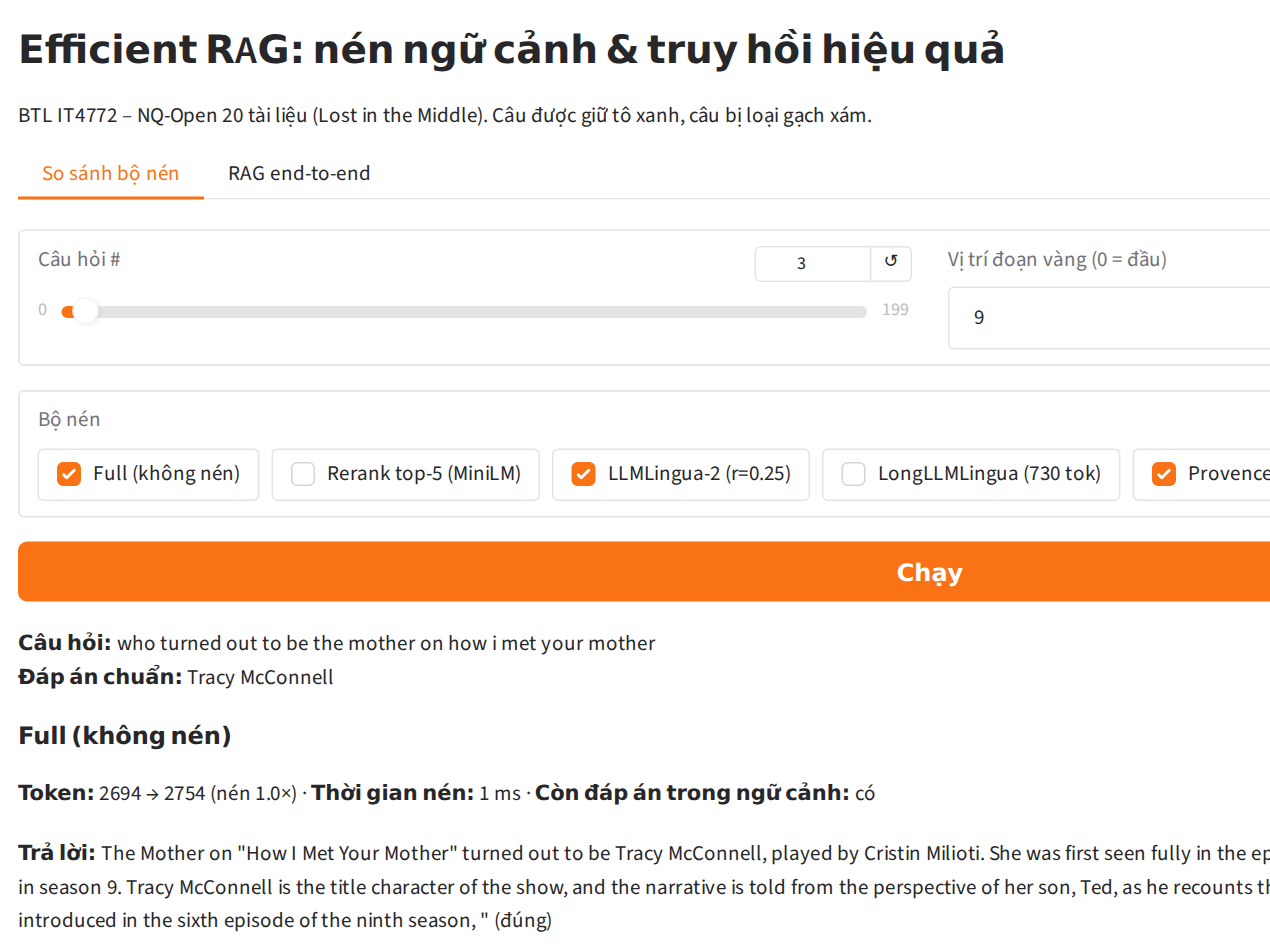
\includegraphics[width=\linewidth]{demo.png}
\caption{Tab ``So sánh bộ nén'' của demo (câu hỏi \#3, đoạn vàng ở vị trí 10, chạy trên CPU).
LLMLingua-2 và Provence đều giữ được đáp án; với Provence, reader 7B trả lời bằng tên diễn viên
(Cristin Milioti) thay vì tên nhân vật -- một kiểu lỗi được phân tích ở Mục~\ref{sec:res-errors}.}
\label{fig:demo}
\end{figure}

\begin{figure}[t]
\centering
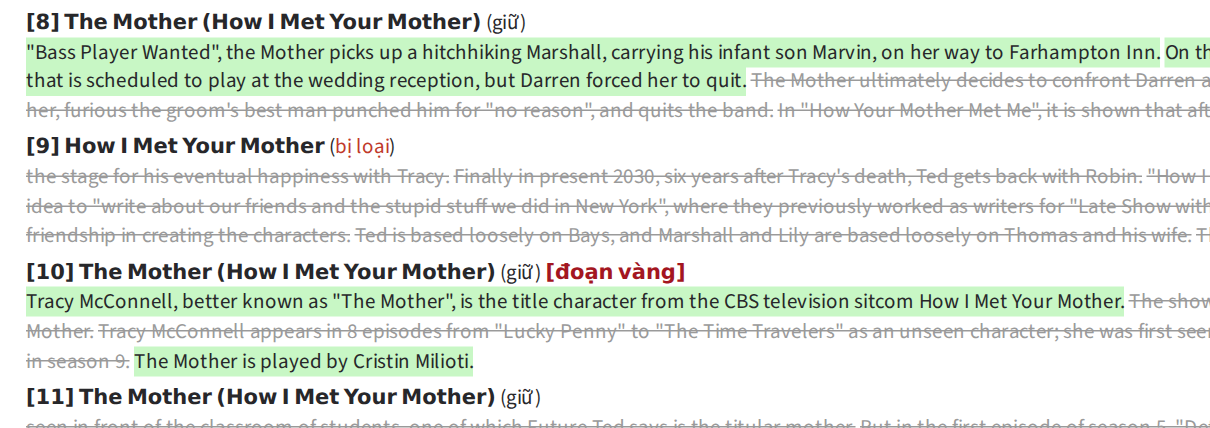
\includegraphics[width=\linewidth]{demo_context.png}
\caption{Ngữ cảnh sau nén của Provence trong demo: câu được giữ (nền xanh), câu bị loại (gạch ngang),
đoạn bị loại hoàn toàn và đoạn vàng.}
\label{fig:demo-context}
\end{figure}
